\documentclass[hidelinks, 11 pt, class=report,crop=false]{standalone}
\usepackage{geometry}
\geometry{verbose,paperwidth=16.1 cm, paperheight=24 cm, inner=2.3cm, outer=1.8 cm, bmargin=2cm, tmargin=1.8cm}
\usepackage[dvipsnames, xetex, table]{xcolor}
\setlength{\parindent}{0bp}
\usepackage{import}
\usepackage[subpreambles=false]{standalone}
\usepackage{amsmath}
\usepackage{amssymb}
\usepackage{esint}

\usepackage{imakeidx}
\makeindex[title=Indeks]

\usepackage[many]{tcolorbox}
\usepackage{mathtools} % for mathclap



% Lister med bokstavar
\usepackage[inline]{enumitem}
\newcounter{rg}
\numberwithin{rg}{chapter}

%referances
\newcommand{\net}[2]{{\color{blue}\href{#1}{#2}}}
\newcommand{\hrs}[2]{\hyperref[#1]{\color{blue}#2 \ref*{#1}}}
\newcommand{\refunnbr}[2]{\hyperref[#1]{\color{blue}#2}}

\newcommand\fork[2]{\begin{tcolorbox}[boxrule=0.3 mm,arc=0mm,enhanced jigsaw,breakable,colback=yellow!7] {\large \textbf{#1 (\expl)} \vspace{5 pt}\\} #2 \end{tcolorbox}\vspace{-5pt} }
\newcommand{\mb}{\net{https://sindrsh.github.io/FirstPrinciplesOfMath/}{MB}}
\newcommand{\reg}[2][]{\begin{tcolorbox}[boxrule=0.3 mm,arc=0mm,colback=blue!3] {\refstepcounter{rg}\phantomsection \large \textbf{\therg \;#1} \vspace{5 pt}}\newline #2  \end{tcolorbox}\vspace{-5pt}}
\newcommand{\regdef}[2][]{\begin{tcolorbox}[boxrule=0.3 mm,arc=0mm,colback=blue!3] {\refstepcounter{rg}\phantomsection \large \textbf{\therg \;#1} \vspace{5 pt}}\newline #2  \end{tcolorbox}\vspace{-5pt}}
\newcommand{\words}[1]{\begin{tcolorbox}[boxrule=0.3 mm,arc=0mm,colback=teal!3] #1  \end{tcolorbox}\vspace{-5pt}}


\newcommand\eks[2][]{\begin{tcolorbox}[boxrule=0.3 mm,arc=0mm,enhanced jigsaw,breakable,colback=green!3] {\large \textbf{\ekstitle #1} \vspace{5 pt}\\} #2 \end{tcolorbox}\vspace{-5pt} }

\newcommand{\st}[1]{\begin{tcolorbox}[boxrule=0.0 mm,arc=0mm,enhanced jigsaw,breakable,colback=yellow!12]{ #1} \end{tcolorbox}}

\newcommand{\spr}[1]{\begin{tcolorbox}[boxrule=0.3 mm,arc=0mm,enhanced jigsaw,breakable,colback=yellow!7] {\large \textbf{\sprtitle} \vspace{5 pt}\\} #1 \end{tcolorbox}\vspace{-5pt} }

\newcommand{\info}[2]{\begin{tcolorbox}[boxrule=0.3 mm,arc=0mm,enhanced jigsaw,breakable,colback=cyan!6] {\large \textbf{#1} \vspace{5 pt}\\} #2 \end{tcolorbox}\vspace{-5pt} }

\newcommand\algv[1]{\vspace{-11 pt}\begin{align*} #1 \end{align*}}


\newcommand\alg[1]{\begin{align*} #1 \end{align*}}
\newcommand{\sym}[1]{\colorbox{blue!15}{#1}}
\newcommand{\regv}{\vspace{5pt}}
\newcommand{\mer}{\textsl{\note}: }
\newcommand{\mers}[1]{{\footnotesize \mer #1}}
\newcommand\vsk{\vspace{11pt}}
\newcommand{\tbs}{\vspace{5pt}}
\newcommand\vs{\vspace{-11pt}}
\newcommand\vsb{\vspace{-16pt}}
\newcommand\br{\\[5 pt]}
\newcommand{\figp}[1]{../fig/#1}
\newcommand\algvv[1]{\vs\vs\begin{align*} #1 \end{align*}}
\newcommand{\y}[1]{$ {#1} $}
\newcommand{\os}{\\[5 pt]}
\newcommand{\prbxl}[2]{
	\parbox[l][][l]{#1\linewidth}{#2
}}
\newcommand{\prbxr}[2]{\parbox[r][][l]{#1\linewidth}{
		\setlength{\abovedisplayskip}{5pt}
		\setlength{\belowdisplayskip}{5pt}	
		\setlength{\abovedisplayshortskip}{0pt}
		\setlength{\belowdisplayshortskip}{0pt} 
		\begin{shaded}
			\footnotesize	#2 \end{shaded}}}
\newcommand{\fgbxr}[2]{
	\parbox[r][][l]{#1\linewidth}{#2
}}		


\usepackage{datetime2}

% outline word
\newcommand{\outl}[1]{{\boldmath \color{teal}\textbf{#1}}}
%line to seperate examples
\newcommand{\linje}{\rule{\linewidth}{1pt} }


\usepackage[]{hyperref}

% arabic language
\usepackage{polyglossia}
\setdefaultlanguage{arabic}
\setmainfont{Amiri}
\newcommand{\note}{ملاحظة}
\newcommand{\notesm}[1]{{\footnotesize \textsl{\note:} #1}}
\newcommand{\ekstitle}{مثال }
\newcommand{\sprtitle}{صندوق اللغة}
\newcommand{\expl}{توضيح}

\newcommand\sv{\vsk \textbf{الإجابة} \vspace{4 pt}\\}

%references
\newcommand{\reftab}[1]{\hrs{#1}{جدول}}
\newcommand{\rref}[1]{\hrs{#1}{قاعدة}}
\newcommand{\dref}[1]{\hrs{#1}{تعريف}}
\newcommand{\refkap}[1]{\hrs{#1}{فصل}}
\newcommand{\refsec}[1]{\hrs{#1}{قسم}}
\newcommand{\refdsec}[1]{\hrs{#1}{قسم فرعي}}
\newcommand{\refved}[1]{\hrs{#1}{ملحق}}
\newcommand{\eksref}[1]{\textsl{#1}}
\newcommand\fref[2][]{\hyperref[#2]{\textsl{شكل \ref*{#2}#1}}}
\newcommand{\refop}[1]{{\color{blue}تمرين \ref{#1}}}
\newcommand{\refops}[1]{{\color{blue}تمرين \ref{#1}}}
\newcommand{\refgrubs}[1]{{\color{blue}تأمل \ref{#1}}}

\newcommand{\openmathser}{\openmath\,-\,السلسلة}

% Exercises
\newcommand{\opgt}{\newpage \phantomsection \addcontentsline{toc}{section}{تمارين} \section*{تمارين للفصل \thechapter}\vs \setcounter{section}{1}}

% Sequences and series
\newcommand{\sumarrek}{مجموع سلسلة حسابية}
\newcommand{\sumgerek}{مجموع سلسلة هندسية}
\newcommand{\regnregsum}{قوانين جمع السلسلة}

% Trigonometry
\newcommand{\sincoskomb}{جمع السين و الكوس}
\newcommand{\cosfunk}{وظيفة الكوسين}
\newcommand{\trid}{هويات تريغونومترية}
\newcommand{\deravtri}{المشتقة للوظائف التريغونومترية}
% Solutions manual
\newcommand{\selos}{انظر إلى الحل المقترح.}
\newcommand{\se}[1]{انظر المثال في الصفحة \pageref{#1}}

%Vectors
\newcommand{\parvek}{متوازي الاتجاهات}
\newcommand{\vekpro}{منتج النواة}
\newcommand{\vekproarvol}{منتج النواة كمساحة وحجم}

% 3D geometries
\newcommand{\linrom}{خط في الفضاء}
\newcommand{\avstplnpkt}{المسافة بين نقطة ومستوى}

% Integral
\newcommand{\bestminten}{التكامل المحدد I}
\newcommand{\anfundteo}{نظرية أساس الأناليز}
\newcommand{\intuf}{تكامل وظائف مختارة}
\newcommand{\bytvar}{تغيير المتغير}
\newcommand{\intvol}{التكامل كحجم}
\newcommand{\andordlindif}{معادلات التفاضل الخطية من الدرجة الثانية}


\begin{document}
\opgt
\setcounter{section}{1}	

\op{odpar}
\textbf{a)} Skriv opp de tre første partallene. Lag en rekursiv og en eksplisitt formel for det $ i $-te partallet.\os
	
\textbf{b)} Skriv opp de tre første oddetallene. Lag en eksplisitt formel for det $ i $-te oddetallet. 

\op{eksar}
Finn det eksplisitte uttrykket til  den aritmetiske følgen når du vet at\os
\begin{tabular}{@{}l l}	
	\textbf{a)} $ a_1=3 $ og $ a_4 = 30 $ \os 
	\textbf{b)} $ a_1 = 5 $ og $ a_{11} = -25 $ \os
	\textbf{c)} $ a_3 =14 $ og $ a_5=26 $ 
\end{tabular}\os

\op{eksgeo}
Finn det eksplisitte uttrykket til den geometriske følgen når du vet at\os
\begin{tabular}{@{}l l}	
	\textbf{a)} $ a_1=\frac{1}{2} $ og $ a_2 = \frac{1}{6} $ \os 
	\textbf{b)} $ a_1 = 5 $ og $ a_4 = 40 $
\end{tabular} \os

\begin{comment}
	\op
Bruk formelen fra oppgave \textsl{\ref{sumkvad}a} og det eksplisitte uttrykket for en aritmetisk følge til å forklare at summen av en aritmetisk rekke kan skrives som:
\[na_1 +\frac{dn(n-1)}{2} \]


\op
a) Bruk (\ref{sumg}) og vis at summen $ S_\infty $ når $ n\to\infty $ blir:
\[ S_\infty=a_1\frac{1}{1-k} \]
for $ |k|<1 $.
\end{comment}
\nes

\op{parodd}
\textbf{a)} Bruk figuren under til å forklare at summen $ S_n $ av de $ n $ første naturlige tallene er gitt ved
\[S_n=\frac{n(n+1)}{2}  \]

\begin{figure}
	\centering
	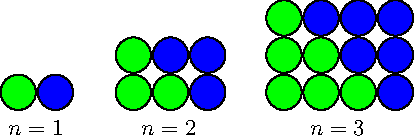
\includegraphics[]{../../fig/sum}
\end{figure}\vs
\textbf{b)} Skriv opp summen av det første, de to første og de tre første  oddetallene. Bruk en lignende figur som i oppgave a) til å vise at summen $ S_n $ av de $ n $ første oddetallene er
\[ S_n = n^2 \] 

\op{opgnegsum}
$ -1-2-3 $ er en rekke. Skriv om rekka slik at den blir uttrykt ved ledd som adderes med hverandre. 

\op{sum10ar}
Finn $ S_{10} $ for rekkene:\os
\begin{tabular}{@{}l l}	
	\textbf{a)} $ 7+13+19+25+\ldots $\quad
	\textbf{b)} $ 1+9+17+25+\ldots $
\end{tabular} \os

\op{ar435}
Gitt rekken 
\[ 8+11+14+\ldots \]
For hvilken $ n $ er summen av rekken lik 435?

\op{opgarekfraeks}
Gitt den uendelige rekken
\[ 3+7+11+... \] 
For hvilken $ n $ er summen av rekken lik 903?

\op{opggerekfraeks}
Gitt den uendelige rekken
\[ 3+6+12+24+... \]	
For hvor mange element er summen av rekken lik 93?

\op{viseks3}
Bruk summen av en aritmetisk rekke til å vise at ligningen gitt i \hyperref[prodind]{\textsl{Eksempel 3}} på s. \pageref{prodind} er sann.

\op{geon}
Gitt rekken
\[ 3+12+48+\ldots+768 \]
Finn summen av rekken. 
\newpage
\op{geoa12}
En geometrisk rekke har $ {a_1 = 2} $ og $ {k=3} $.\os 

\textbf{a)} Vis at summen $ S_n $ kan skrives som:
\[ S_n = 3^n-1 \]
\textbf{b)} Regn ut summen for de tre første leddene.\os

\textbf{c)} For hvilken $ n $ er $ S_n=728 $?



\begin{comment}
\textbf{c)} Hvis du fortsetter å spare slik, og medregner innskudd samme måned, når vil du ha 24200 kr på konto? 
\end{comment}

\op{1over4}
Gitt den uendelige rekken
\[ 4+1+\frac{1}{4}+\ldots \]
\textbf{a)} Forklar hvorfor rekken er konvergent.\os

\textbf{b)} Finn summen av den uendelige rekken.

\op{opggerekuendeks}
Gitt den uendelige rekka 
\[ 1+\frac{1}{x}+\frac{1}{x^2}+.... \]
\abc{
\item  For hvilken $ x $ er summen av rekka lik $ \frac{3}{2} $?\os

\item For hvilken $ x $ er summen av rekka lik $ -1 $?
}

\begin{comment}
	\op{stav} 
	Tenk at uendelig mange personer skal sette sammen en stav. Første person legger på en meter, neste person legger på 0.1 m, neste legger på 0.01 m osv. Hvor lang blir staven?
\end{comment}
\newpage
\op{099er1}
\textbf{a)} Skriv det uendelige desimaltallet 0.999... som en uendelig geometrisk rekke.\os

\textbf{b)} Forklar hvorfor rekken er konvergent og bruk dette faktumet til å finne summen av rekken. 

\op{geokonv}
Gitt den uendelige rekken
\[\frac{1}{3} +\frac{1}{3}(x-2)+ \frac{1}{3}(x-2)^2+\ldots\]
\textbf{a)} For hvilke $ x $ er rekken konvergent? \os

\textbf{b)} For hvilken $ x $ er $ S_n = \frac{2}{9} $?\os

\textbf{c)} For hvilken $ x $ er $ S_n= \frac{1}{6}$? \os

\nes
\op{ind}
Vis ved induksjon at for alle $ n\in \mathbb{N} $ er\\[10pt]
\begin{tabular}{@{}l l}	
	\textbf{a)} $ 1+2+3+\ldots+n = \dfrac{n(n+1)}{2} $ \\[10pt]
	\textbf{b)} $ 1+2 +2^2 +\ldots+ 2^{n-1}= 2^n-1$\\[10pt]
	\textbf{c)} $ 4+4^2+4^3+\ldots+4^n = \dfrac{4}{3}(4^n-1) $ \\[10pt]
	\textbf{d)} $ 1^2 + 2^2+3^2+ \ldots+ n^2 = \dfrac{n(2n+1)(n+1)}{6} $ 
\end{tabular} 

\op{div3}
Vis ved induksjon at $ n(n^2+2) $ er delelig med 3 for alle $ n\in\mathbb{N} $.

\op{factorials}
\textbf{a)}
Vis ved induksjon at:
\[\frac{1\cdot2}{1}\cdot\frac{1\cdot2\cdot3\cdot4}{1\cdot2\cdot3}\cdot
\ldots\cdot\frac{(2n)!}{(2n-1)!}=2^n n! \]
\textsl{Hint}: \y{(2(k+1))!=(2k+1)!(2k+2)}.\os

\textbf{b)} Hvordan kan venstresiden i a) skrives enklere? Utfør induksjonsbeviset på nytt etter forenklingen.
\newpage
\grubop{opgsumnkvad}
Måletl med denne oppgaven er å, uten bruk av induksjon, vise at summen av $ n $ kvadrater er gitt ved følgende formel:
\[ \sum\limits_{i=1}^n i^2 = \frac{n(2n+1)(n+1)}{6} \tag{I}\label{sumkvad}\]
\textbf{a)} Forklar hvorfor vi kan skrive
\[ 1^2 + 2^2 + 3^2+\ldots = 1 + (1+3) + (1+3+5)+ \ldots  \]
\textsl{Hint}: se opg. \ref{parodd} b).\os

\textbf{b)} Ut ifra det du fant i a), forklar at
\[ \sum\limits_{i=1}^n i^2 = n+\sum\limits_{i=1}^n (n-i)(2i+1)  \]
\textbf{c)} Skriv ut alle kjente summer fra b) og løs ligningen med hensyn på $ \sum\limits_{i=1}^n i^2 $, du skal da komme fram til (\ref{sumkvad}).
\end{document}
\begin{comment}
\op{eksplar}
Finn det eksplisitte uttrykket til den aritmetiske rekken når du vet at:
\os
\begin{tabular}{@{}l l}	
\textbf{a)} $ a_1=-5 $ og $ a_8=44 $. \os 
\textbf{b)} $ a_7=39 $ og $ d=6 $. \os
\textbf{c)} $ a_5 = 16 $ og $ a_{10} = 31 $
\end{tabular}
\end{comment}